\chapter{Concepción y Diseño}\label{chapter:proposal}

A partir de las ideas adquiridas con el estudio de las herramientas expuestas en el cap\'itulo \ref{chapter:auto-etl}, 
en el presente capítulo se aborda el diseño de un lenguaje de dominio específico para la definición de 
escenarios analíticos. Asimismo, se expone la concepción general del marco de trabajo \textbf{AutoETL} para la 
integración de datos de forma automática partiendo de un modelo analítico definido mediante el DSL, cuya estructura 
f\'isica almacenar\'a los datos integrados. Los escenarios analíticos que se definen son esquemas estrellas, que como 
se expuso en el cap\'itulo \ref{chapter:teoricframe} especifican las dimensiones y las tablas de hechos 
que conforman un almacén de datos. 

Las dimensiones, generalmente, están formadas por atributos de distintas tablas de
las fuentes de datos, por ejemplo, una dimension que expresa la ubicación geográfica
se forma mediante el join de las tablas municipio, provincia y país. En las bases de
datos relacionales con un diseño correcto, es usual encontrarse estos tres conjuntos de
entidades separados en tablas normalizadas, enlazadas mediante llaves foráneas, con
el objetivo de evitar duplicación de datos y anomalías durante la inserción, modificación
y eliminación. Por tanto, el proceso de selección de datos para la población de la
dimensión ubicación geográfica pasa por la ejecuci\'on de joins sobre las tablas municipio, provincia y país,
para poder extraer los datos desde una única tabla, es decir, denormalizar la red  
de tablas municipio, provincia y país que fue formada durante el proceso de normalización. 

En las tabla de hechos sucede algo similar, puede que los valores de un hecho se
encuentren en una sola tabla o que en su calculo intervengan atributos de múltiples
tablas de la fuente, en ese caso es necesario interrelacionar explícitamente todas las tablas que intervengan
en el cálculo del hecho en cuestión mediante joins.

Luego una parte fundamental del proceso de integración de datos para la población de un escenario analítico es
la implementación de estos joins. Precisamente, la inferencia de joins por parte del marco trabajo concebido es el centro de atención de la presente 
investigaci\'on. La inferencia de joins implica la identificaci\'on mediante algoritmos y el uso de estructuras de datos de 
las tablas que intervienen en una consulta y las condiciones de join entre dichas tablas.
AutoETL realiza el proceso de inferencia de joins durante la generaci\'on 
del c\'odigo SQL asociado a las consultas que poblar\'an el escenario analítico, apoy\'andose de la definición del mismo
mediante el lenguaje de dominio específico.

\section{Concepción y Diseño}\label{section:design}

\begin{figure}
    \centering
    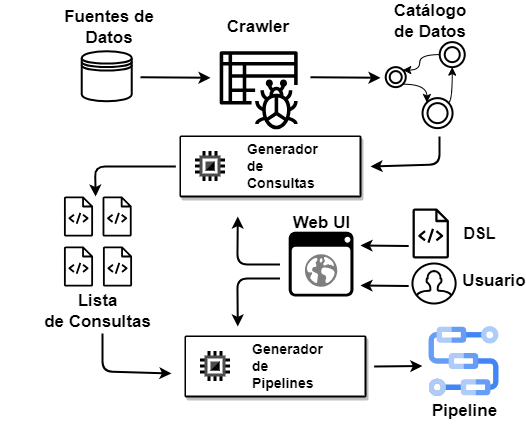
\includegraphics[width=0.60\textwidth]{Graphics/arch.drawio.png}
    \caption{Arquitectura del prototipo de AutoETL}
    \label{fig:arquitectura}
    \end{figure}

AutoETL se concibe como una herramienta para ser utilizada por los desarrolladores de almacenes de datos 
con el objetivo de aliviar la carga de trabajo en la implementaci\'on de los procesos de población de las 
estructuras analíticas. Como se observa en la Figura \ref{fig:arquitectura} los componentes de la aplicaci\'on 
est\'an dispuestos de forma secuencial para representar el flujo de trabajo de la herramienta.

